%&platex --translate-file=cp1250pl
\documentclass[times]{jtitauth}

\begin{document}

\title{Sensitivity of the Impact Factor\\
with Respect to Alterations in Publication Year\\
}

\author{Nicholas Rose,  Varan Culanathan, and Shlomo Zilberstein}

\markboth{Nicholas Rose,  Varan Culanathan, and Shlomo Zilberstein}
{Sensitivity of the Impact Factor with Respect to Alterations in Publication Year}

\maketitle

\begin{abstract}
The impact factor has recently gained popularity as a mechanism to measure the success of a journal. The formula, although simple, has been studied by many to determine its validity, accuracy, and ability to be manipulated. One unexplored area of the impact factor is its sensitivity in regards to a shift in publication year. One key way in which the publication year of a paper can be altered is by being unofficially available online for up to a year before being officially published in a journal. We cite journals that are known to follow such practices and attempt to find the effect of such practices on the impact factor of a journal. Our goal was to obtain a database of papers from a journal that is known not to alter the publication year in any way, and emulate a scenario where the publication year is altered. By obtaining papers published in the Journal of Artificial Intelligence from the years of 1999-2013 through Google Scholar, we were able to calculate the impact factor for the journal using data from Google Scholar. We were then able to calculate the impact factor for every year if papers published in the journal had their year of publication shifted by one year, and analyze the results of doing so. In this paper, we hypothesize that by shifting the year of publication of papers in a journal by one year, the impact factor will be positively influenced.     
\end {abstract}

\begin{keywords}
impact factor, Google Scholar, JAIR, sensitivity, citations, publications, scientometrics
\end{keywords}

\section{Introduction}


Many methods exist in the status quo to measure the reputability and success of publishing journals, but just a few gain widespread use by journals of the 21st century. One of the most notable of these methods is the impact factor, a measure used by many journals largely for citation analysis. This measurement has grown to become one of the most influential tools in modern research and academia despite its simplicity. 

The impact factor for a journal can be calculated by obtaining two elements: the number of citations in a given year from works published in in the previous two years, and the number of works published in those same two years. It is important to note that all works being used to calculate the impact factor come solely from works published in the journal for which the impact factor is being calculated for. By dividing the number of citations in a given year from works published in the previous two years by the number of works in the previous two years, the impact factor can be derived.

There are many that criticize the formula used to calculate the impact factor, claiming that it can be manipulated in inappropriate ways, that it improperly influences the publication strategies of scientists, and that the measure itself is not indicative of a journal’s true impact in the scientific community. Given these flaws and more, however, the impact factor is still viewed by many as the standard indicator for a journal’s prestige and visibility.

In this paper, we focus on the sensitivity of the impact factor with respect to a shift in the year of publication. We present a model that could potentially be used to increase the impact factor of a journal by altering the year of publication of papers within a given journal. By simulating a scenario where the year of publication of all papers in a journal are delayed for a single year while maintaining the same amount of exposure, we find that this can drastically increase the impact factor of a journal. Observing a data set of over 700 papers from a single journal, we find results that prove our methods of alteration to the publication year consistently produce a higher impact factor for a journal. 

Over the course of data collection and analysis, we realize the simplicity and effectiveness of altering the publication year of papers in a journal. We hypothesize that delaying the publication year of papers within a journal while maintaining the same amount of visibility can positively influence the impact factor of a journal. From our results, we attempt to quantify the effect to the impact factor by delaying the publication years of papers. With the resulting dataset, we provide some analysis of trends in impact factor growth from our experiments.


\section{Experimental Setup}
\subsection {Data Collection}
To conduct our experiment, we gathered a dataset consisting of papers published in the Journal of Artificial Intelligence. Through efficient crowd-sourcing techniques using the Amazon Mechanical Turk platform, we obtained the citation information of 755 papers, which accounted for every paper published in the Journal of Artificial Intelligence between 1999 and 2015. Our dataset was collected from citation data published freely on Google Scholar. We found Google Scholar to be the most effective platform to gather the necessary citation data. One reason we found Google Scholar to be a reliable source was because it has gained a reputation for having far greater retroactive growth than many other databases for papers while also covering a larger scope of papers than other databases (Winser et. al). By sending out microtasks on Amazon Mechanical Turk, we had workers fill out the citation information for each paper in the journal over the allotted 17 years. 
\begin{figure}[!hbp]
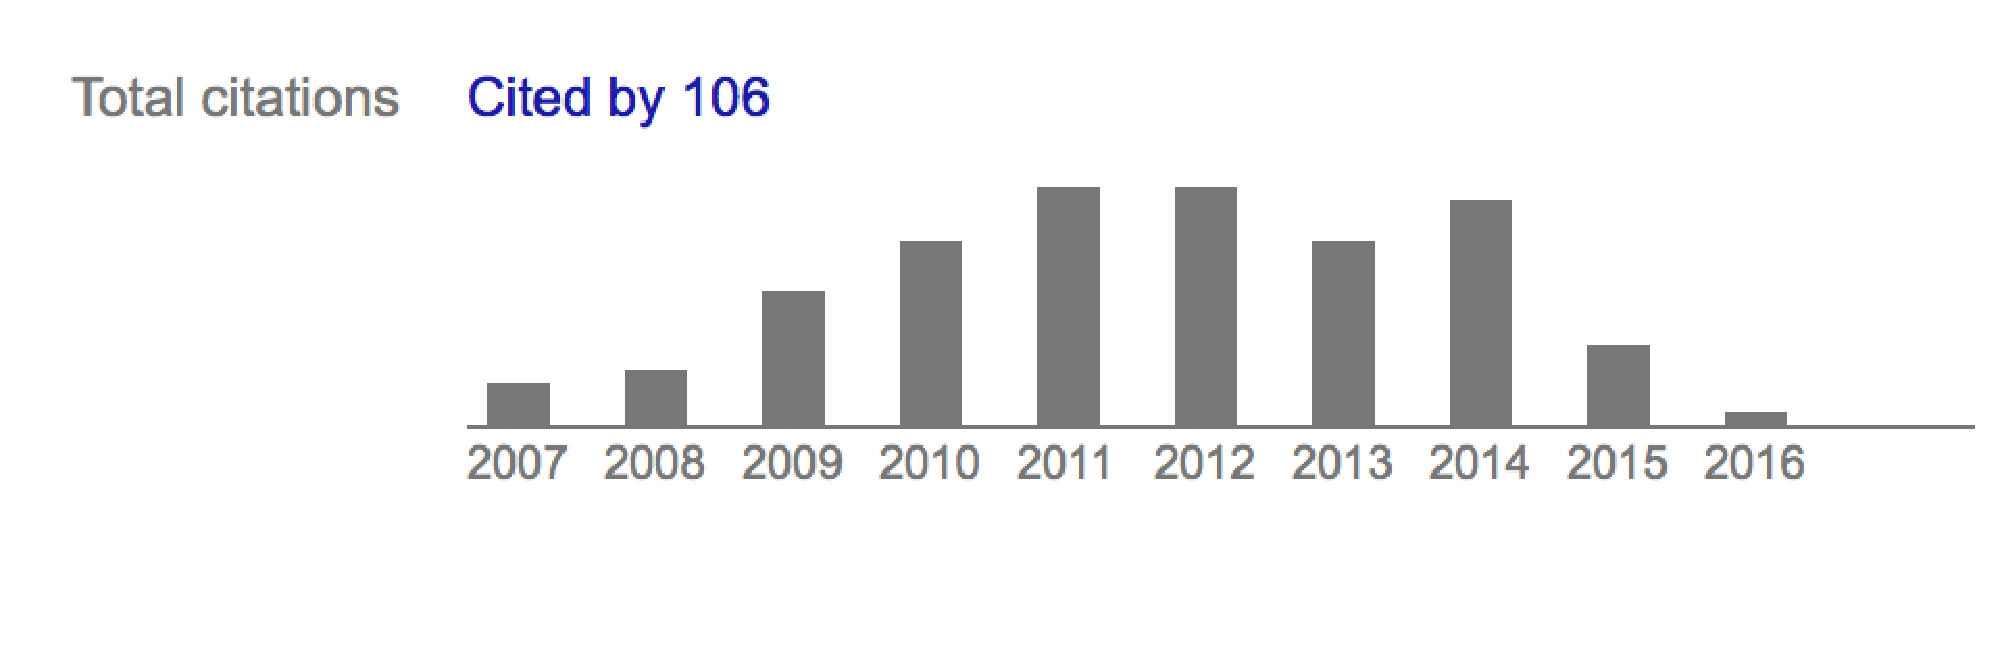
\includegraphics[scale=0.25]{fig}
\caption{Example histogram of citations from Google Scholar for a paper}
\end{figure}

Figure 1 shows a histogram for a paper published in 2007 from which citation data would be obtained by workers on Mechanical Turk. Hovering over each bar of the histogram, the number of citations appear for that year. 
\subsection{Experiment}
After obtaining our dataset, we calculated the impact factor for the years of 2002 - 2013. The impact factor for a given year was calculated using the following formula: 

\begin{equation}
IF =  \frac{A + B}{C+D} 
\end{equation}
\noindent in which\\


\textit{A} = \# of citations papers published one year before received in a given year
\\ \textit{B} = \# of citations papers published two years before received in a given year
\\ \textit{C} = \# of papers published one year before given year 
\\ \textit{D} = \# of papers published two years before given year \\ 

For example, to calculate the impact factor for the year 2009 for a journal, the following data would be required:
\\
\\The number of citations that papers published in 2007 received in 2009 
\\The number of citations that papers published in 2008 received in 2009 
\\The number of papers published in 2007
\\The number of papers published in 2008 \\

Using the citation data from the model paper (see Fig. 1), in order to calculate the impact factor for 2009, the number of citations that this paper received in 2009 would be used. The number of citations that this paper received was 10. 

For our baseline experiment, we calculated the impact factor as it normally would have been by a journal for all the papers in the Journal of Artificial Intelligence. 

Our interest in the impact factor stems from its potential mutability based on natural trends of a paper's citations. We observe that in a large number of cases, papers receive more citations three years following its year of publication compared to the number of citations it receives two years following its year of publication. In the case of the model paper (see Fig. 1), the number of citations this paper received in 2010 was 14, compared to only 10 in 2009. 

To form our hypothesis as to the sensitivity of the impact factor, we made one key assumption. We assumed that if a paper's year of publication was shifted by one year, but it was freely available before it was published, then it would have the same amount of exposure for the first year as it would if it were published. An example of this would be if a paper was unofficially released in the year 2004 and officially published in 2005 while maintaining the same amount of exposure in both years. 

To produce a dataset of impact factors based on a shift of one year, we used the same dataset as the baseline. Although we used the same formula to calculate the impact factor, the following alterations were made to the variables: \\


\textit{A} = \# of citations papers published two years before received in a given year
\\ \textit{B} = \# of citations papers published three years before received in a given year
\\ \textit{C} = \# of papers published two years before given year 
\\ \textit{D} = \# of papers published three years before given year \\

For example, to calculate the impact factor for the year 2010 for a journal, the following data would be required:\\ \\ 
The number of citations that papers published in 2006 received in 2010 
\\The number of citations that papers published in 2007 received in 2010 
\\The number of papers published in 2006
\\The number of papers published in 2007 \\

The reason for which the papers used in calculating impact factor are shifted backwards a year is because we assume that for the first year a paper is released, it obtains the same amount of exposure without being published. 

\section{Results}
\begin{center}
 \begin{tabular}{| c | c | c | c |} 
 \hline
 Year & Impact Factor & Shifted Impact Factor & Percent Change \\ 
 \hline\hline
 2002 & 7.02 & 10.35 & 47.35\%\\ 
 \hline
 2003 & 7.61 & 9.82 & 29.05\%\\
 \hline
 2004 & 8.59 & 10.15 & 18.15\%\\
 \hline
 2005 & 8.96 & 11.07 & 23.52\%\\
 \hline
 2006 & 8.19 & 11.22 & 36.93\%\\ 
 \hline
 2007 & 7.09 & 10.10 & 42.35\%\\ 
 \hline
 2008 & 8.12 & 9.17 & 12.97\%\\ 
 \hline
 2009 & 6.73 & 9.13 & 35.67\%\\ 
 \hline
 2010 & 7.86 & 8.84 & 12.48\%\\ 
 \hline
 2011 & 8.85 & 9.84 & 11.11\%\\ 
 \hline
 2012 & 6.16 & 10.58 & 71.88\%\\ 
 \hline
 2013 & 4.91 & 8.10 & 64.90\%\\ 
 \hline
\end{tabular}

\end{center}
\textbf{\textit{Fig.2.}}\hspace{.1cm} Experimental data results


\section{Discussion} 
\subsection{Analysis of Results}

After analyzing our dataset, we found that the influence of shifting the impact factor was both positive and consistent across every year examined. We found that on average, the shifted impact factor was 33.86\% higher than the normal impact factor, or an average increase of 2.36. While our dataset came from a single journal, we believe these results can be cross-applied across all journals. This is primarily because publication methods for journals that do not alter a paper's date of publication undergo very similar processes. Although our experiment did not control for exposure, we believe that many tactics can be used by journals to maintain effectively the same amount of exposure as a published paper while not being officially published. While we cannot provide a motive for such actions, we observe that journals such as the Journal of Autonomous Agents and Multi-Agent Systems and the Journal of Automated Reasoning release papers unofficially as "Online First" for up to a year before being published. Based on our research, we believe that such techniques can artificially increase the impact factor of a journal. 

Although the impact factor when shifted never went down, we found that for some years, the impact factor when shifted was much larger than other years. Part of the reason for this was due to the success of certain papers published in JAIR in some years compared to the success of papers published in other years. Although the magnitude of the change varied from year to year, in all our years of study, we found a consistent increase in the impact factor when the year of publication for the papers was shifted.

\subsection{Threats to Validity}
One concerning issue in our methodology was that the official publication of a paper allows for a physical copy of the paper to be distributed, which could increase the number of citations a paper receives in comparison to an online version. In our study, the journal we used to gather citation data for does not have a physical copy, thereby eliminating the influence of citations accruing from a physical copy of papers. To cross apply our results to other journals, we assume that journals that could be affected by this shift in publication year receive a very nominal number of citations from people reading the physical copy of papers.   

Another potential issue stemmed from our use of Google Scholar to collect citation data. Many find data displayed on Google Scholar to be unreliable or innacurate due to imperfections in their scraping methods and poor cleaning of data. Contrary to the belief of critics, recent research has found that Google Scholar has proven to have a far greater breadth, more retroactive growth, and more citations than other major databases. Because of this, we found that Google Scholar could be used reliably in order to find accurate data on paper citations. 



In many cases, papers that are published in conferences or displayed on the author's web page are not officially published until years later. Once the paper is available to everyone, whether through a conference publication or through the author's web page, it may start receiving citations. This can then effect the number of citations that paper later contributes to the impact factor of its journal, but when calculating the impact factor, it does not matter where and how people find papers to cite. In our study, we simply assumed all outside factors remained equal and calculated the shifted impact factor as if each paper would receive the same citations from each source with the one year shift in publication date. 

\begin{center}
\begin{tabular}{| c | c |} 
 \hline
 Year & Impact Factor\\ 
 \hline\hline
 2002 &  0.933\\ 
 \hline
 2003 &  1.615\\
 \hline
 2004 &  2.045\\
 \hline
 2005 &  2.247\\
 \hline
 2006 &  1.795\\ 
 \hline
 2007 &  1.107\\ 
 \hline
 2008 &  1.611\\ 
 \hline
 2009 &  1.981\\ 
 \hline
 2010 &  1.691\\ 
 \hline
 2011 &  1.143\\ 
 \hline
 2012 &  1.056\\ 
 \hline
 2013 &  0.904\\ 
 \hline
\end{tabular}
\end{center}
\textbf{\textit{Fig.3.}}\hspace{.1cm} Official Impact Factor as provided by ResearchGate.\\


Using Google Scholar as the source for citation data, we observed that GS collects more citations than is used to calculate the official impact factor, available of ResearchGate. We believe that the reason for this differential is because GS has a more expansive dataset of publications. Papers that may have been missed or deemed unofficial by those calculating the official impact factor may have been included in Google Scholar's dataset, resulting in a higher amount of papers and more citations to each paper. In our results, the impact factor that we calculated was, on average, about 529\% larger than the official impact factor for that year. 



\section*{Acknowledgements}


\begin{thebibliography}{99}
\bibitem{1}K. R. Wilson and V. V. Yakovlev, "Ultrafast rainbow: tunable ultrashort
 pulses from a solid-state kilohertz system", {\it J. Opt. Soc. Am. B}, vol. 14, pp. 444--448, 1997.
\bibitem{2}J. Comly and E. Garmire, ,,Second harmonic generation from short
pulses'', {\it Appl. Phys. Lett.}, vol. 12, no. 7-9, 1968.
\bibitem{3}O. E. Martinez, ,,Achromatic phase matching for second harmonic ge\-neration
of femtosecond pulses'', {\it IEEE J. Quant. Electron.}, vol.
QE-25, pp. 2464--2468, 1989.

\end{thebibliography}
\end{document}